\documentclass[a4paper,12pt]{article}

\input{packages}

\begin{document}

\subsubsection{Théorème 1}
\begin{theorem}
Deux triangles dont les côtés sont respectivement parallèles ont des angles respectivement isométriques.
\end{theorem}

\begin{proof}
Nous considérons deux triangles quelconques $\triangle ABC$ et $\triangle A'B'C'$.



\begin{figure}[H]
        \centering
        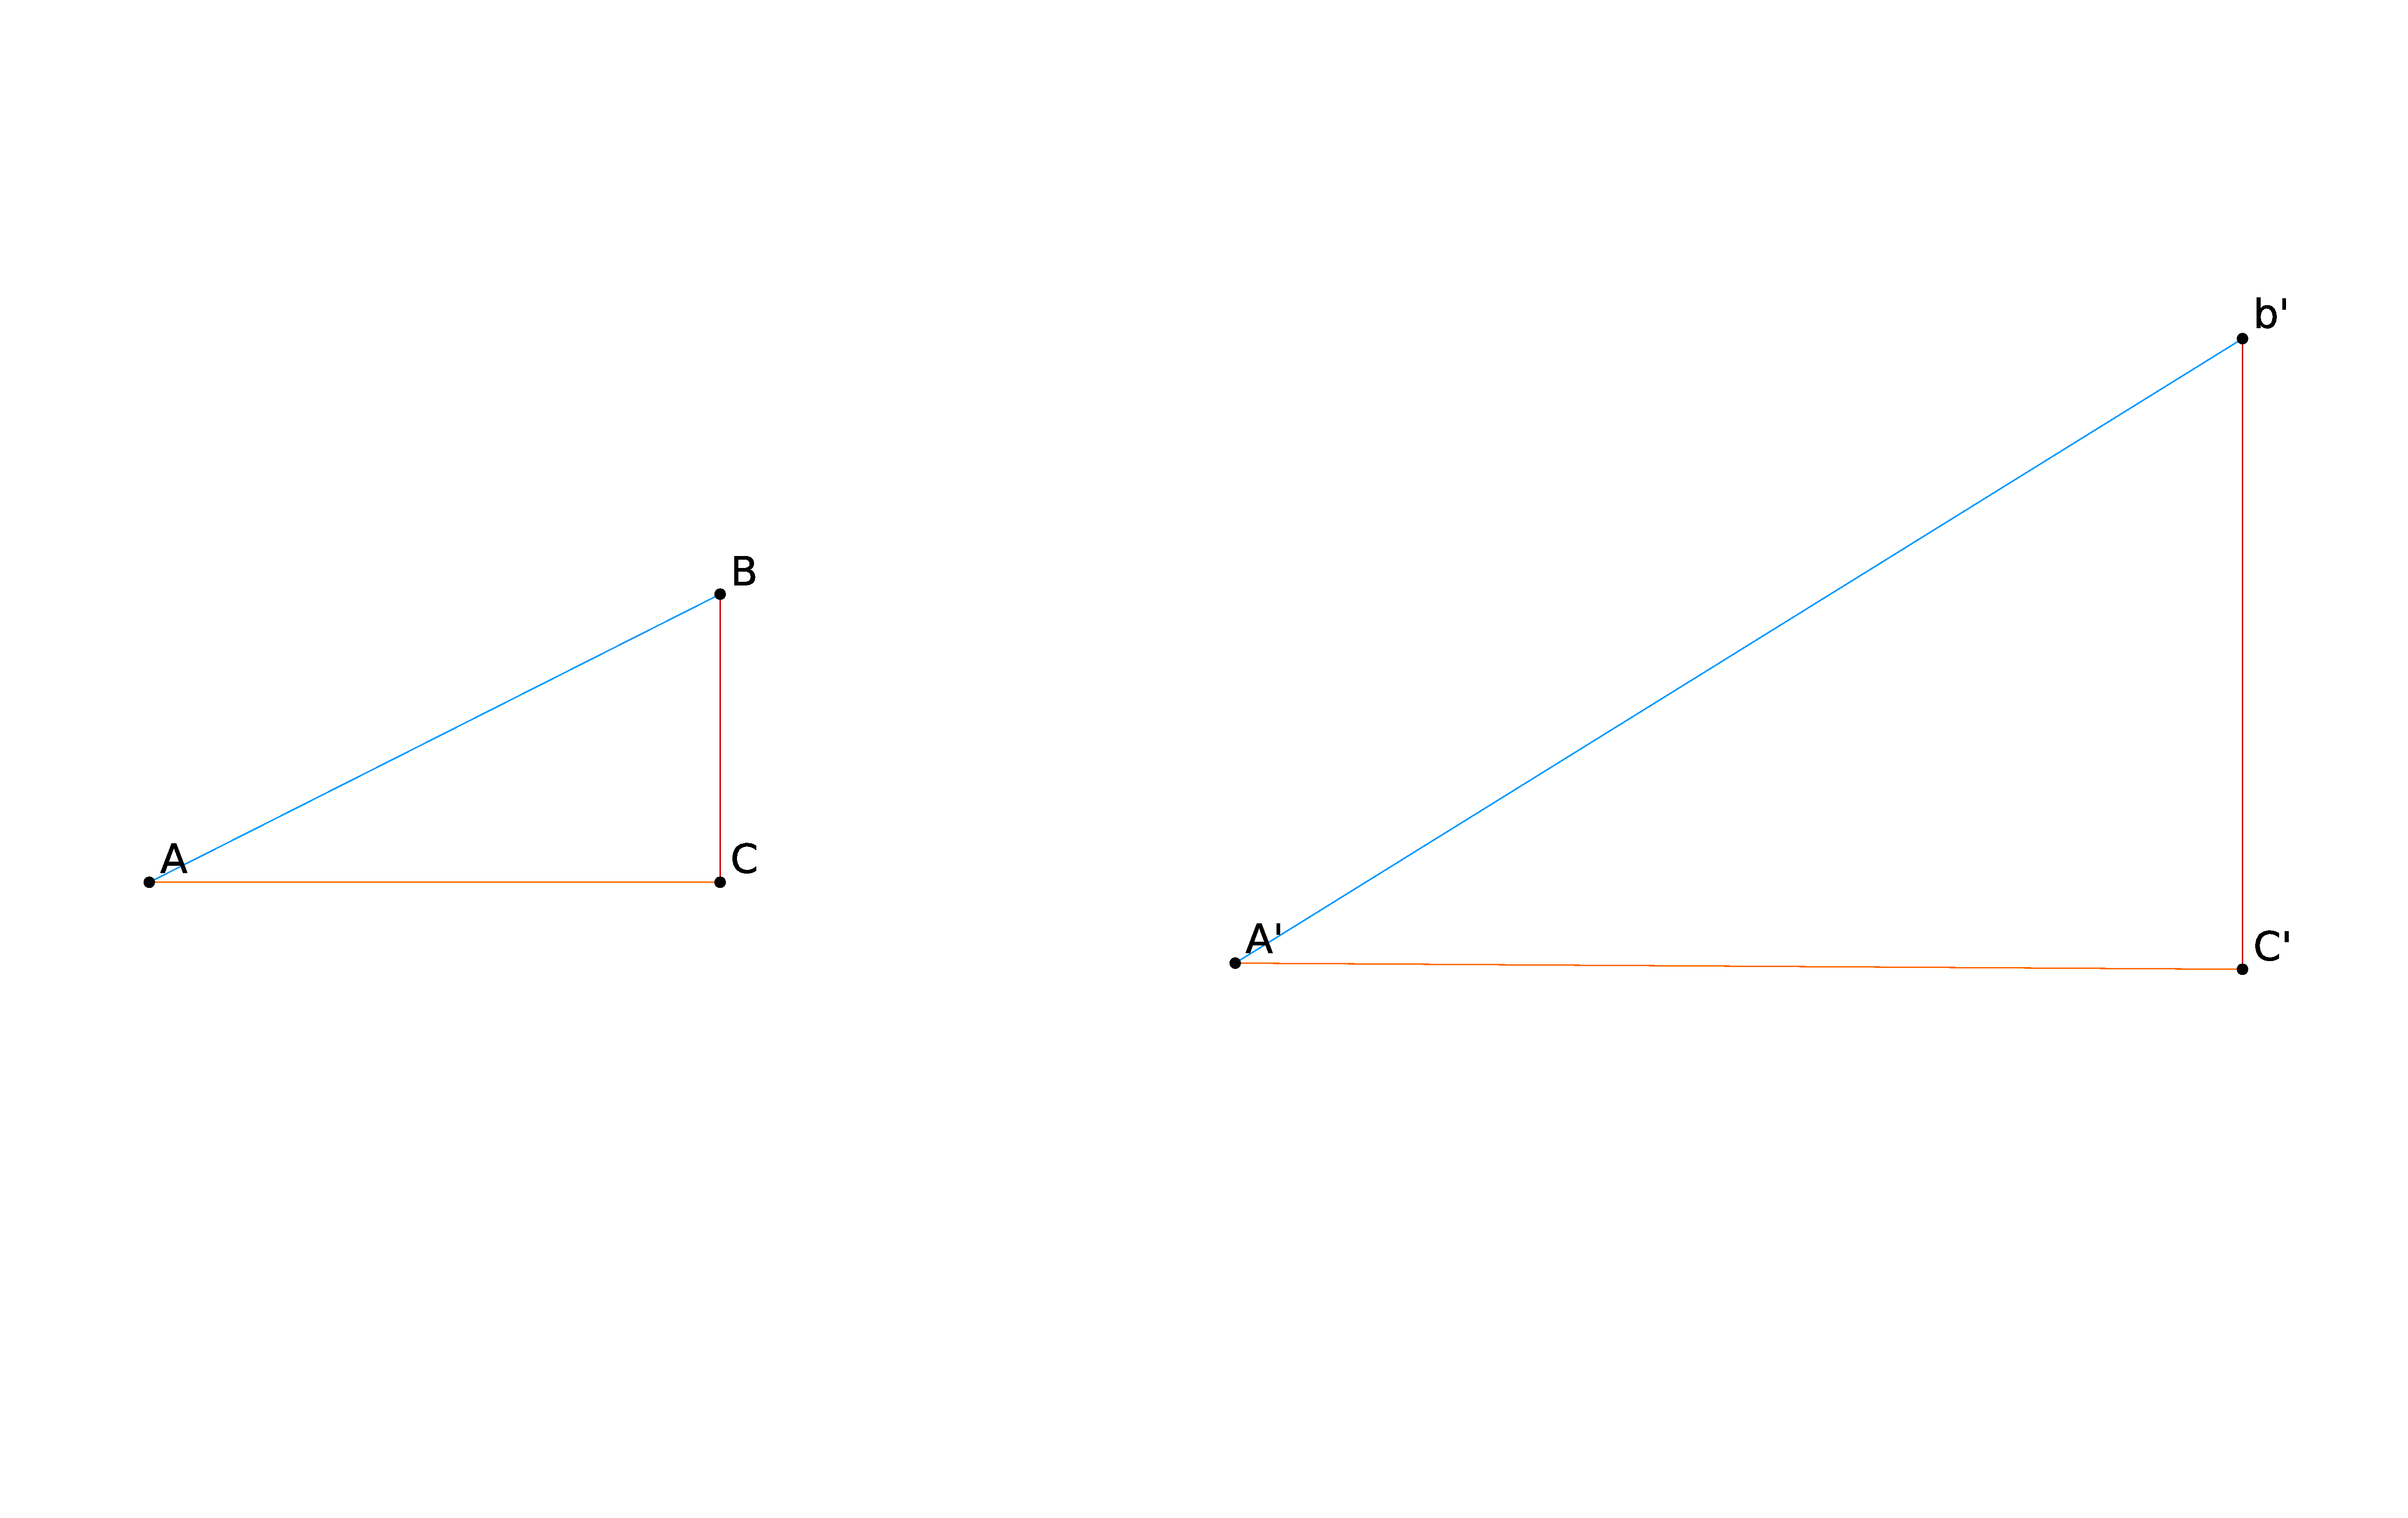
\includegraphics[scale=0.2]{semblable1.1.eps}
    \end{figure}

\begin{hyp}
$a \parallel a'$, $b \parallel b'$ et $c \parallel c'$
\end{hyp}
\begin{concl}
$\alpha \equiv \alpha'$, $\beta \equiv \beta'$ et $\gamma \equiv \gamma'$
\end{concl}

Nous prolongeons $a$, $a'$ et $c'$. 

\begin{figure}[H]
        \centering
        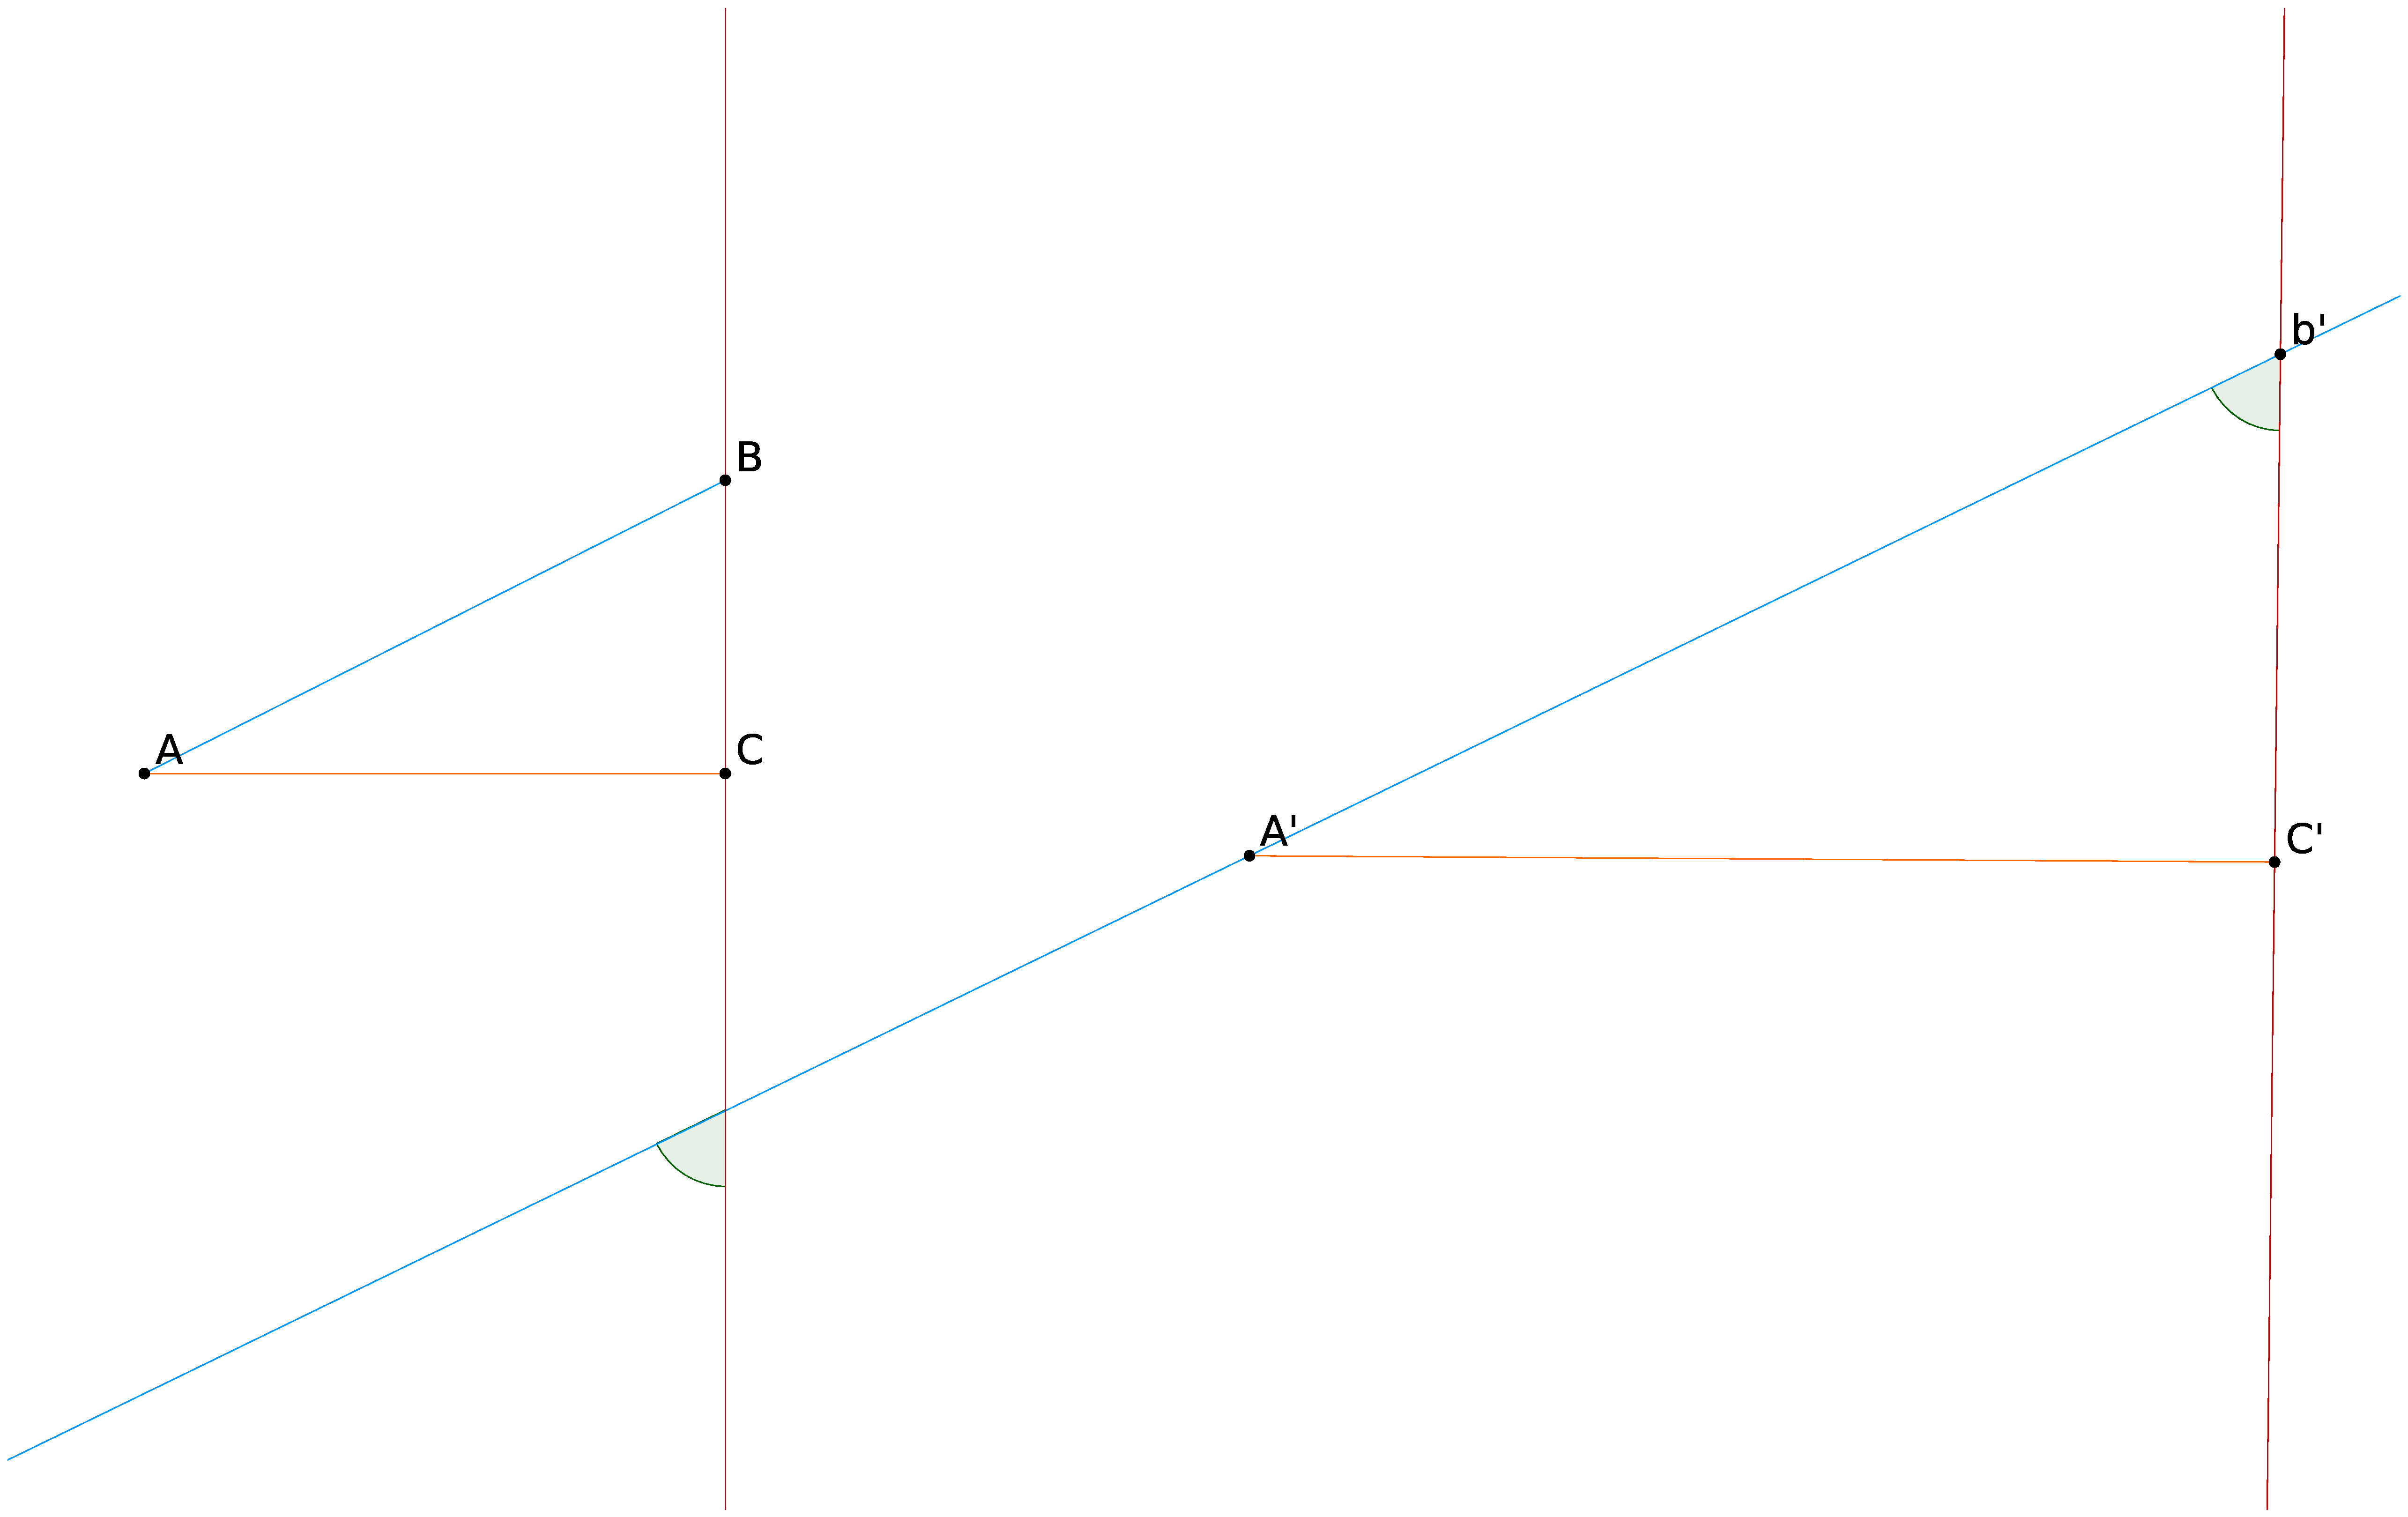
\includegraphics[scale=0.2]{semblable1.2.eps}
    \end{figure}

Grâce au théorème de la transversale, nous observons que $\beta' \equiv \theta$, où theta est l'angle correspondant de beta.\\
Nous prolongeons $c$, $c'$ et $a$ et grâce au même théorème qu'auparavant, nous savons que $\beta \equiv \theta$.
Ainsi, $\beta \equiv \beta' \equiv \theta$.\\
Il suffit de répéter cette démonstration pour les deux autres angles des triangles afin d'obtenir $\alpha \equiv \alpha'$, $\beta \equiv \beta'$ et $\gamma \equiv \gamma'$.

\begin{figure}[H]
        \centering
        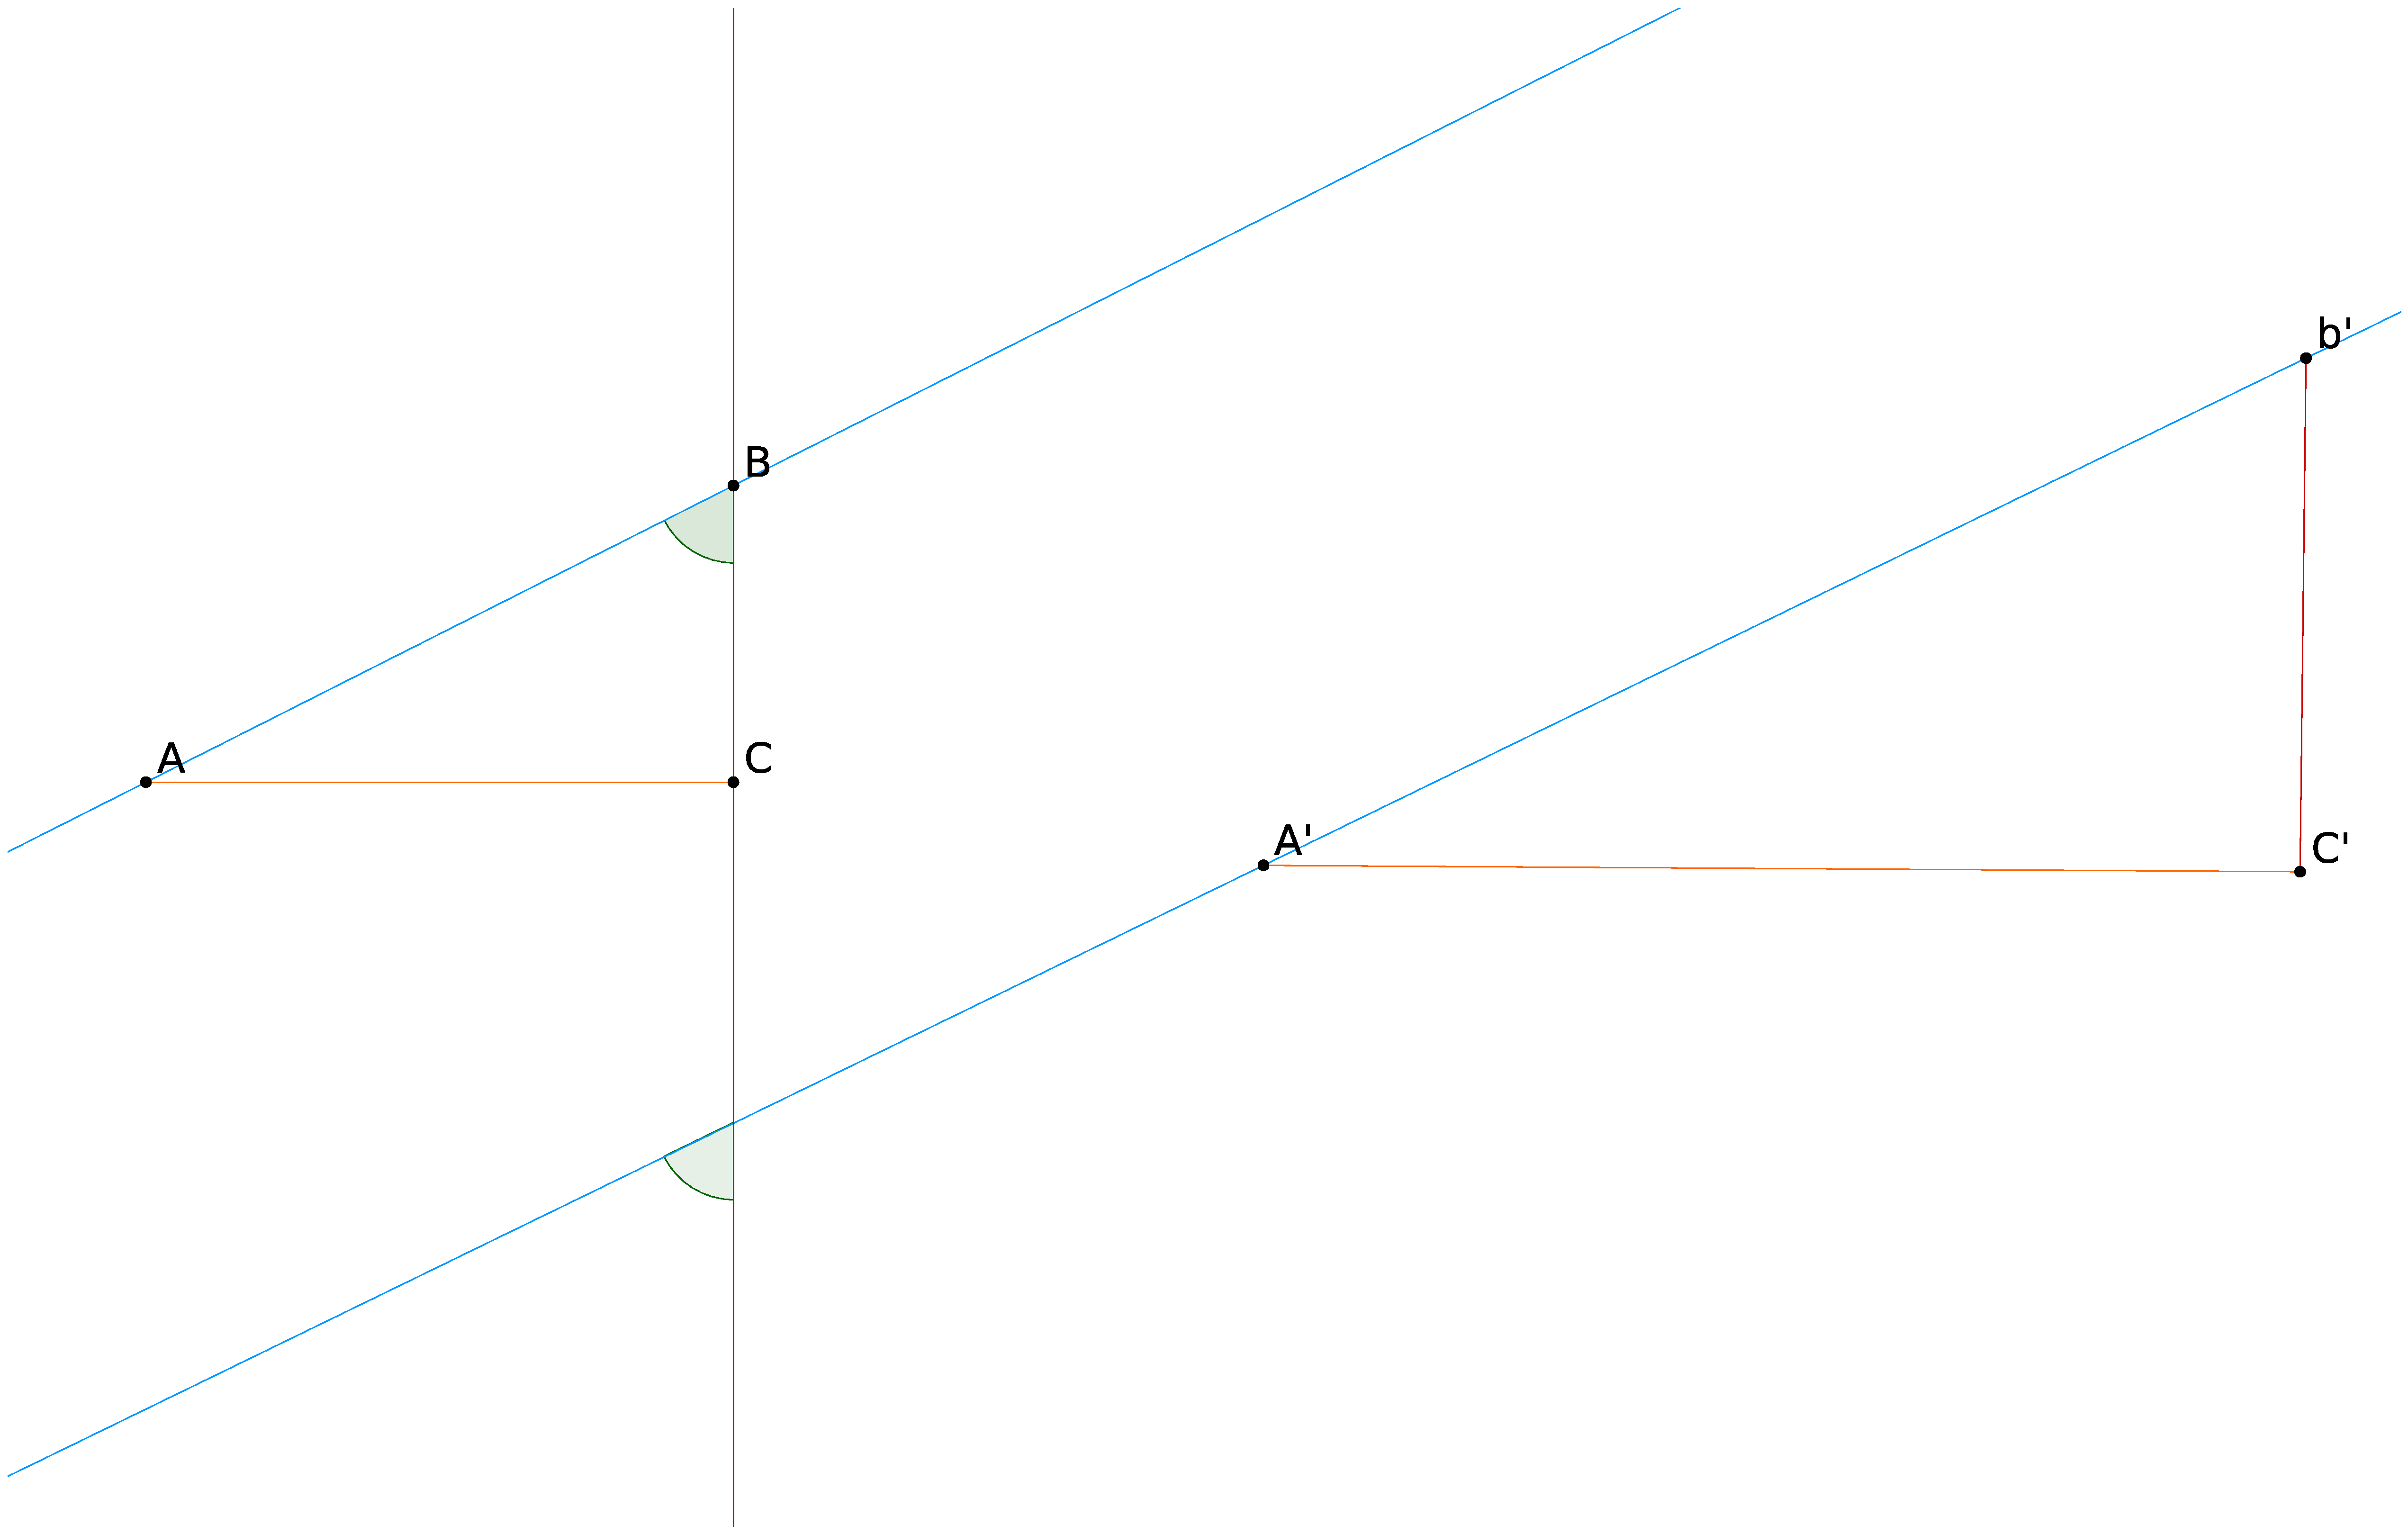
\includegraphics[scale=0.2]{semblable1.3.eps}
    \end{figure}

\end{proof}

\end{document}